\begin{figure}[htb]
	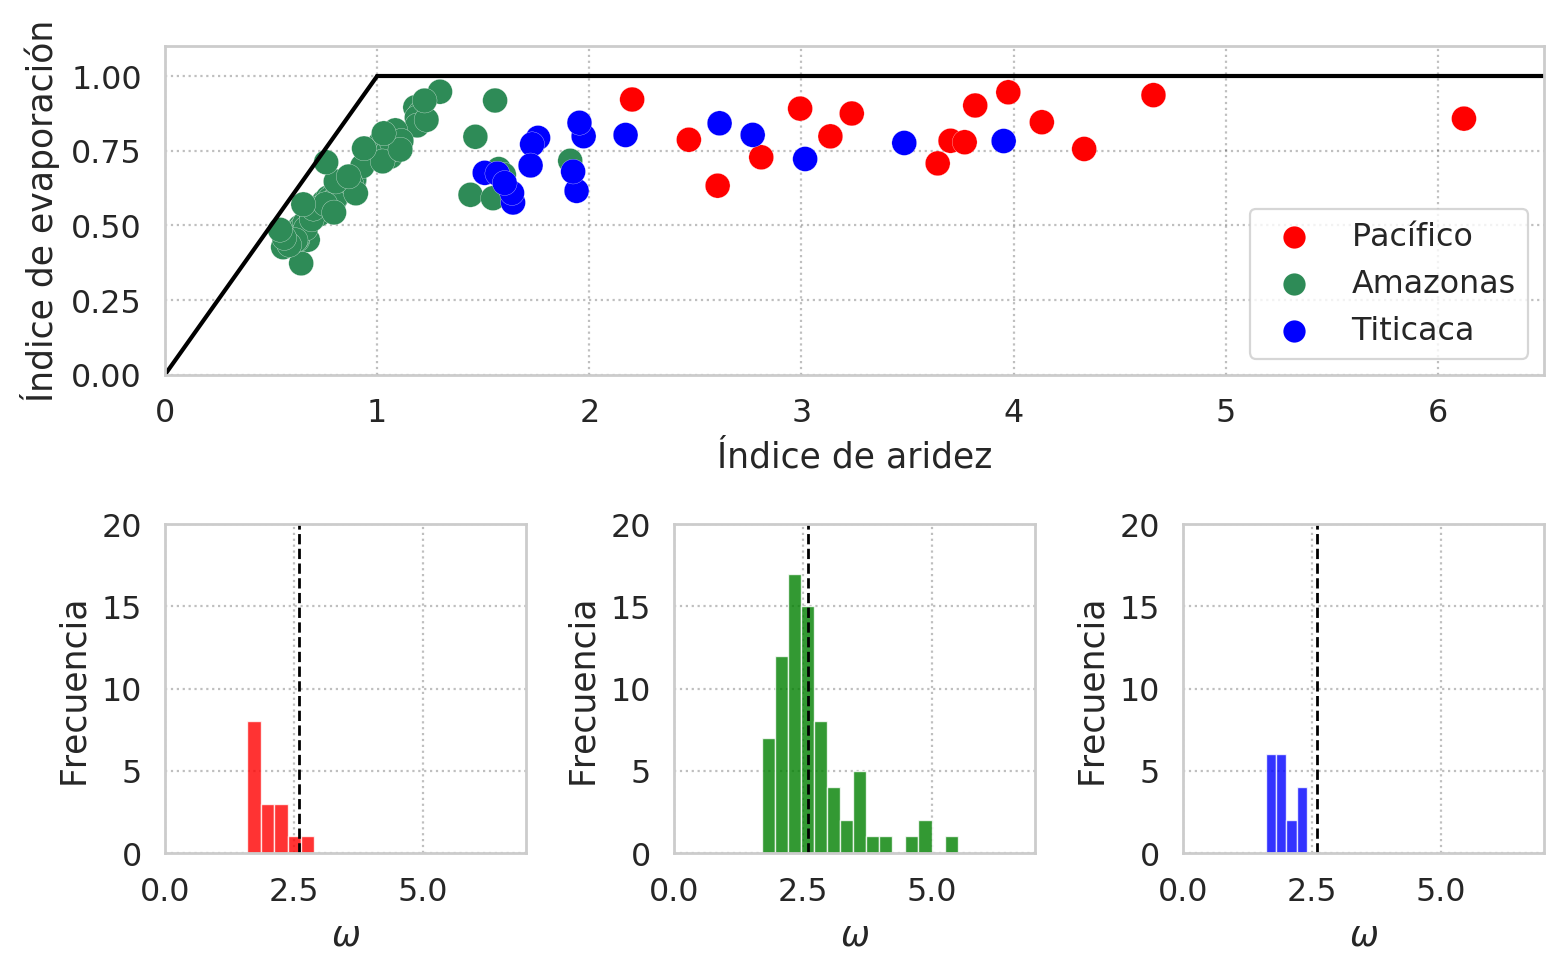
\includegraphics[scale=.78]{Images/07_Curve_and_omega.png}
	\centering
	\caption{Arriba) Ubicación de las UH en la curva de Budyko en función del índice de evaporación ($AE/P$) y aridez ($PE/P$). Abajo) Histogramas de la distribución del parámetro $\omega$ calibrado para cada UH y vertiente. La linea punteada en cada histograma indica el valor teórico de $\omega = 2.6$.}
	\label{fig:07_Curve_and_omega}
\end{figure}
